\section{Search for same-sign dileptons with $b$ jets}
\label{sec:searchbtag}

This analysis is based on the same-sign dilepton search documented in AN-2011/258~\cite{ssnote2011} and corresponds to an
integrated luminosity of 349 pb$^{-1}$. In that study we searched for events with two isolated same-sign leptons
in association with 2 additional jets and \met. Here we re-use most of the baseline event selection~\footnote{The additional 
$Z$ veto is not applied in this study} as summarized in Section~\ref{sec:eventsel} below. 
In addition, we require at least 2 b-tagged jets using Track Counting High Efficiency 
Medium (TCHEM) working point tagger~\cite{BTVPAS2011}. We refer to TCHEM with the requirement that three of the tracks have $IP$ 
significance $ > 3.3$. For this tagger the expected b-tagging efficiency is 62\% with a roughly 20\% systematic uncertainty.
The acceptance of light flavor jets is $\sim 2$\%~\cite{BTVPAS2011}.

\subsection{Event Selection}
\label{sec:eventsel}

As mentioned previously, this search is a refinement of~\cite{ssnote2011}, and we thus discuss here only differences and briefly summarize the basic kinematics and triggers.
For more details, we refer to~\cite{ssnote2011}.

\begin{itemize}
\item We separately look at the dilepton triggerred and dilepton plus $H_T$ triggered samples.
\item At least two isolated same-sign leptons ($ee$, $e\mu$, and $\mu\mu$) with $|\eta| < 2.4$.
\item For the dilepton triggered samples, we require one lepton with $p_T>$20 GeV and a second lepton with $p_T >$10 GeV. We refer to this as the ``high-$p_T$ analysis".
\item For the dilepton plus $H_T$ triggered sample, we require electrons with $p_T>$10 GeV and muons with $p_T >$5 GeV. We refer to this as the ``low-$p_T$ analysis".
\item At least two particle flow jets tagged using TCHEM tagger with $p_T > 40$ GeV and $|\eta| < 2.4$
%{\it why not 3.0 ??} 
corrected with L1FastL2L3 corrections.
\item The selected jets must be separated from the lepton by $\Delta R > 0.4$.
\item \met $> 30$ GeV.
\item We remove dilepton events with invariant mass $M_{ll} < 5$ GeV.
%{\it switched to tighter mll cut because we can.}
\end{itemize}

More details are found in Reference~\cite{ssnote2011}.

\subsection{Event Yields and Background Estimation}
\label{eventsel}

The results of this search in the above-mentioned kinematical region are summerized in Table~\ref{tab:ssyields1}.
As mentioned in the introduction, and quantified by this table, SM background is expected to be dominated by $t\bar{t}$ production
with one real and one fake lepton.
We estimate this background from the data itself using the ``Tight-To-Loose ratio'' (Fake Rate) method~\cite{frmethod}.
Electron charge mis-reconstruction is estimated by weighting opposite-sign dilepton events that pass all our cuts
by a charge flip rate obtained form single electron Monte Carlo as described in detail in~\cite{ssnote2011}.
The probability for muons to be reconstructed with the wrong sign in the relevant momemtum range is negligible.
Both of these techniques are described in more detail in~\cite{ssnote2011}.
Systematic errors on these two estimates are 50\% and 25\% respectively.

In addition, we use MC to estimate contributions from the following additional SM production processes.
All of these are quite small.

\begin{itemize}
\item $qqW^\pm W^\pm, WWW, t\bar{t}W$, and double parton $W^\pm W^\pm$ with two real leptons in the final state.
\item $WZ$ and $ZZ$ with two real leptons in the final state.
\item $W\gamma$ with one real lepton and a photon conversion. This background is a priori not estimated by the fake rate method
because the photon is generally isolated. In practice, this background is completely negligible.
\end{itemize}

{\it Need to update the tables to include the remaining MC bkg as the MC becomes available !!!}

%\vspace{6 mm}
\begin{table}[htb]
\begin{center}
\begin{tabular}{|c|c|c|c|c|}
\hline
Sample & $e^{\pm}e^{\pm}$    & $\mu^{\pm}\mu^{\pm}$ & $e^{\pm}\mu^{\pm}$      & total \\ \hline
% all the MCs
\hline
\ttbar  & 0.15 $\pm$ 0.09 & 0.25 $\pm$ 0.11 & 0.25 $\pm$ 0.11 & 0.65 $\pm$ 0.18 \\ 
Single top  & 0.02 $\pm$ 0.02 & 0.02 $\pm$ 0.02 & 0.02 $\pm$ 0.01 & 0.06 $\pm$ 0.03 \\ 
wjets  & 0.00 $\pm$ 0.00 & 0.00 $\pm$ 0.00 & 0.00 $\pm$ 0.00 & 0.00 $\pm$ 0.00 \\ 
DY  & 0.00 $\pm$ 0.00 & 0.00 $\pm$ 0.00 & 0.00 $\pm$ 0.00 & 0.00 $\pm$ 0.00 \\ 
VV  & 0.00 $\pm$ 0.00 & 0.00 $\pm$ 0.00 & 0.00 $\pm$ 0.00 & 0.00 $\pm$ 0.00 \\ 
\hline
Total MC  & 0.17 $\pm$ 0.09 & 0.27 $\pm$ 0.11 & 0.27 $\pm$ 0.11 & 0.71 $\pm$ 0.18 \\
\hline\hline
data  (349 pb$^{-1}$)     & 1  &  1  & 0  & 2      \\ \hline
fake rate prediction & & & & \\ \hline
single fake   & 0.38 $\pm$ 0.38 & 0.52 $\pm$ 0.37 & 0.00 $\pm$ 0.00 & 0.90 $\pm$ 0.52 (3 evts) \\
double fake   & 0.00 $\pm$ 0.00 & 0.00 $\pm$ 0.00 & 0.00 $\pm$ 0.00 & 0.00 $\pm$ 0.31 (0 evts) \\
fake prediction & 0.38 $\pm$ 0.38 & 0.52 $\pm$ 0.37 & 0.00 $\pm$ 0.00 & 0.90 $\pm$ 0.60 \\
\hline\hline
flip rate prediction & $0.05 \pm 0.01$ & 0 & $0.06\pm 0.02$ & $0.11\pm 0.03$ \\ \hline
total fake rate prediction & $0.38 \pm 0.43$ & $0.52\pm 0.45$ & $0.00 \pm 0.00$ & $0.90 \pm 0.69$ \\ \hline
total bkg prediction & $0.43\pm 0.43$ & $0.52 \pm 0.45$ & $0.06 \pm 0.2$ & $1.01\pm 0.75$ \\\hline
\end{tabular}
\caption{\protect Data and Monte Carlo yields for the same-sign high-$p_T$ dileptons with $H_T > 80$ GeV and \met $> 30$ GeV. Uncertainties in 
the lower three rows also include the systematic uncertanities on the method used.\label{tab:ssyields1} }
\end{center}
\end{table}

%\vspace{6 mm}
\begin{table}[htb]
\begin{center}
\begin{tabular}{|c|c|c|c|c|}
\hline
Sample & $e^{\pm}e^{\pm}$    & $\mu^{\pm}\mu^{\pm}$ & $e^{\pm}\mu^{\pm}$      & total \\ \hline
% all the MCs
\hline
\ttbar  & 0.15 $\pm$ 0.09 & 0.25 $\pm$ 0.11 & 0.30 $\pm$ 0.19 & 0.70 $\pm$ 0.19 \\ 
Single top  & 0.02 $\pm$ 0.02 & 0.02 $\pm$ 0.02 & 0.02 $\pm$ 0.01 & 0.06 $\pm$ 0.03 \\ 
wjets  & 0.00 $\pm$ 0.00 & 0.00 $\pm$ 0.00 & 0.00 $\pm$ 0.00 & 0.00 $\pm$ 0.00 \\ 
DY  & 0.00 $\pm$ 0.00 & 0.00 $\pm$ 0.00 & 0.00 $\pm$ 0.00 & 0.00 $\pm$ 0.00 \\ 
VV  & 0.00 $\pm$ 0.00 & 0.00 $\pm$ 0.00 & 0.00 $\pm$ 0.00 & 0.00 $\pm$ 0.00 \\ 
\hline
Total MC  & 0.17 $\pm$ 0.09 & 0.27 $\pm$ 0.11 & 0.32 $\pm$ 0.19 & 0.76 $\pm$ 0.19 \\
\hline\hline
data  (349 pb$^{-1}$)     & 0  &  1  & 0  & 1      \\ \hline
fake rate prediction & & & & \\ \hline
single fake   & 0.00 $\pm$ 0.00 & 0.00 $\pm$ 0.00 & 0.00 $\pm$ 0.00 & 0.00 $\pm$ 0.56 (0 evts) \\
double fake   & 0.00 $\pm$ 0.00 & 0.51 $\pm$ 0.30 & 0.00 $\pm$ 0.00 & 0.51 $\pm$ 0.30 (3 evts) \\
fake prediction & 0.00 $\pm$ 0.00 & 0.51 $\pm$ 0.30 & 0.00 $\pm$ 0.00 & 0.51 $\pm$ 0.63 \\
\hline\hline
flip rate prediction & $0.01 \pm 0.004$ & 0 & $0.02\pm 0.006$ & $0.03\pm 0.01$ \\ \hline
total fake rate prediction & $0.00 \pm 0.00$ & $0.51\pm 0.68$ & $0.00 \pm 0.00$ & $0.51 \pm 0.68$ \\ \hline
total bkg prediction & $0.01\pm 0.004$ & $0.51 \pm 0.68$ & $0.02 \pm 0.006$ & $0.54 \pm 0.68$ \\\hline
\end{tabular}
\caption{\protect Data and Monte Carlo yields for the same-sign low-$p_T$ dileptons with $H_T > 200$ GeV and \met $> 30$ GeV. Uncertainties in 
the lower three rows also include the systematic uncertanities on the method used.\label{tab:ssyields2} }
\end{center}
\end{table}

The estimation
is in a good agreement with the observation. We also note that the backgrounds with respect to the inclusive same-sign
dilepton search is suppressed by an order of magnitude due to the b-tag requirements.

We have visually scanned all the events in data and provide details in Section~\ref{sec:inclresults}.

%{\it We need to add this still in the results section !!!}

\subsection{Discussion of Background Expectation From MC}
\label{sec:bkgdiscussion}

Three MC studies are presented. First, we show the origin of fake leptons in MC.
Second, we 
show explicitly the degree to which the fake rate method
accurately predicts the fake lepton background in \ttbar MC, 
and third, we present evidence for our assertion that a b-quark can not simultaneously provide a b-tag and produce a fake lepton.

We use a large \ttbar sample~\footnote{The POWHEG sample TTToLNu2Q2B\_7TeV-powheg-pythia6\_Spring11-PU\_S1\_START311\_V1G1-v1 } 
normalized to 1~fb$^{-1}$ for these studies. 
The fake rates were obtained from QCD MC as described in detail in~\cite{ssnote2011}.

We classify \ttbar background events based on truth matching to their ``parent parton''
as either ``Heavy Flavor" or ``Light Flavor". Charm quarks from W decay are classified as heavy flavor.
It is thus possible to have three heavy quarks in the same event, one of which provides the isolated lepton,
the two others the b-tags.

As is shown in Table~\ref{tab:fakeOrigin1}  about 60\% (40\%) of the fake leptons are from heavy (light) flavor.

%{\it\bf Need to sort out how much of the HF contribution is in events with W to charm decays !!! I.e. where %does the remaining
%heavy flavor bkg come from?} 

\begin{table}[hbt]
\begin{center}
\begin{tabular}{|l|c|c|c|}\hline
Same Sign Leptons & Total  & Heavy Flavor & Light Flavor  \\ \hline

$ee$ & 0.31$\pm$0.07 &  0.11$\pm$0.04 & 0.21$\pm$0.05  \\
$\mu\mu$ & 0.26$\pm$0.06 & 0.22$\pm$0.05 & 0.04$\pm$0.04 \\
$e\mu$ & 0.57$\pm$0.09 & 0.37$\pm$0.07 & 0.21$\pm$0.05 \\
total & 1.15$\pm$0.13 & 0.70$\pm$0.10 & 0.45$\pm$ 0.08 \\ \hline
\end{tabular}
\caption{ Expected number of \ttbar events in 1 fb$^{-1}$ of integrated luminosity. Uncertainties are from MC statistics.\label{tab:fakeOrigin1}}
\end{center}
\end{table}

Table~\ref{tab:fakeOrigin2} shows the same breakdown for the fake rate prediction.
Here we use an MC sample where one of the W's is forced to decay leptonically while the other is not allowed to decay
leptonically.
We use this sample as it has x10 the luminosity equivalent than the standard \ttbar sample, thus providing higher statistics for 
this test. We observe an overprediction of 30\% which appears to be primarily due to overpredicting the fakes from heavy flavor.

\begin{table}[hbt]
\begin{center}
\begin{tabular}{|l|c|c|c|}\hline
Same Sign Leptons & Total &  Heavy Flavor & Light Flavor\\ \hline
$ee$ & 0.39$\pm$0.03 & 0.20$\pm$0.02 & 0.19$\pm$0.03 \\
$\mu\mu$ & 0.36$\pm$0.03 & 0.30$\pm$0.03 & 0.06$\pm$0.01 \\
$e\mu$ & 0.76$\pm$0.05 & 0.54$\pm$0.04 & 0.22$\pm$0.03 \\
total & 1.51$\pm$0.06 & 1.04$\pm$0.05 & 0.47$\pm$0.04  \\ \hline
\end{tabular}
\caption{ Predicted number of \ttbar events in 1 fb$^{-1}$ of integrated luminosity. Uncertainties are from MC statistics.\label{tab:fakeOrigin2}}
\end{center}
\end{table}

Finally, Figure~\ref{fig:ttbar_residual} shows the minimum $\Delta R$ between one of the two b-tagged jets and 
the fake lepton in the MC after 
relaxing the jet veto cone around the lepton. 
The black line indicates the jet veto cone size. Clearly, a b-quark can not simultaneously provide a b-tag and an isolated lepton.

\begin{figure}[htb]
\begin{center}
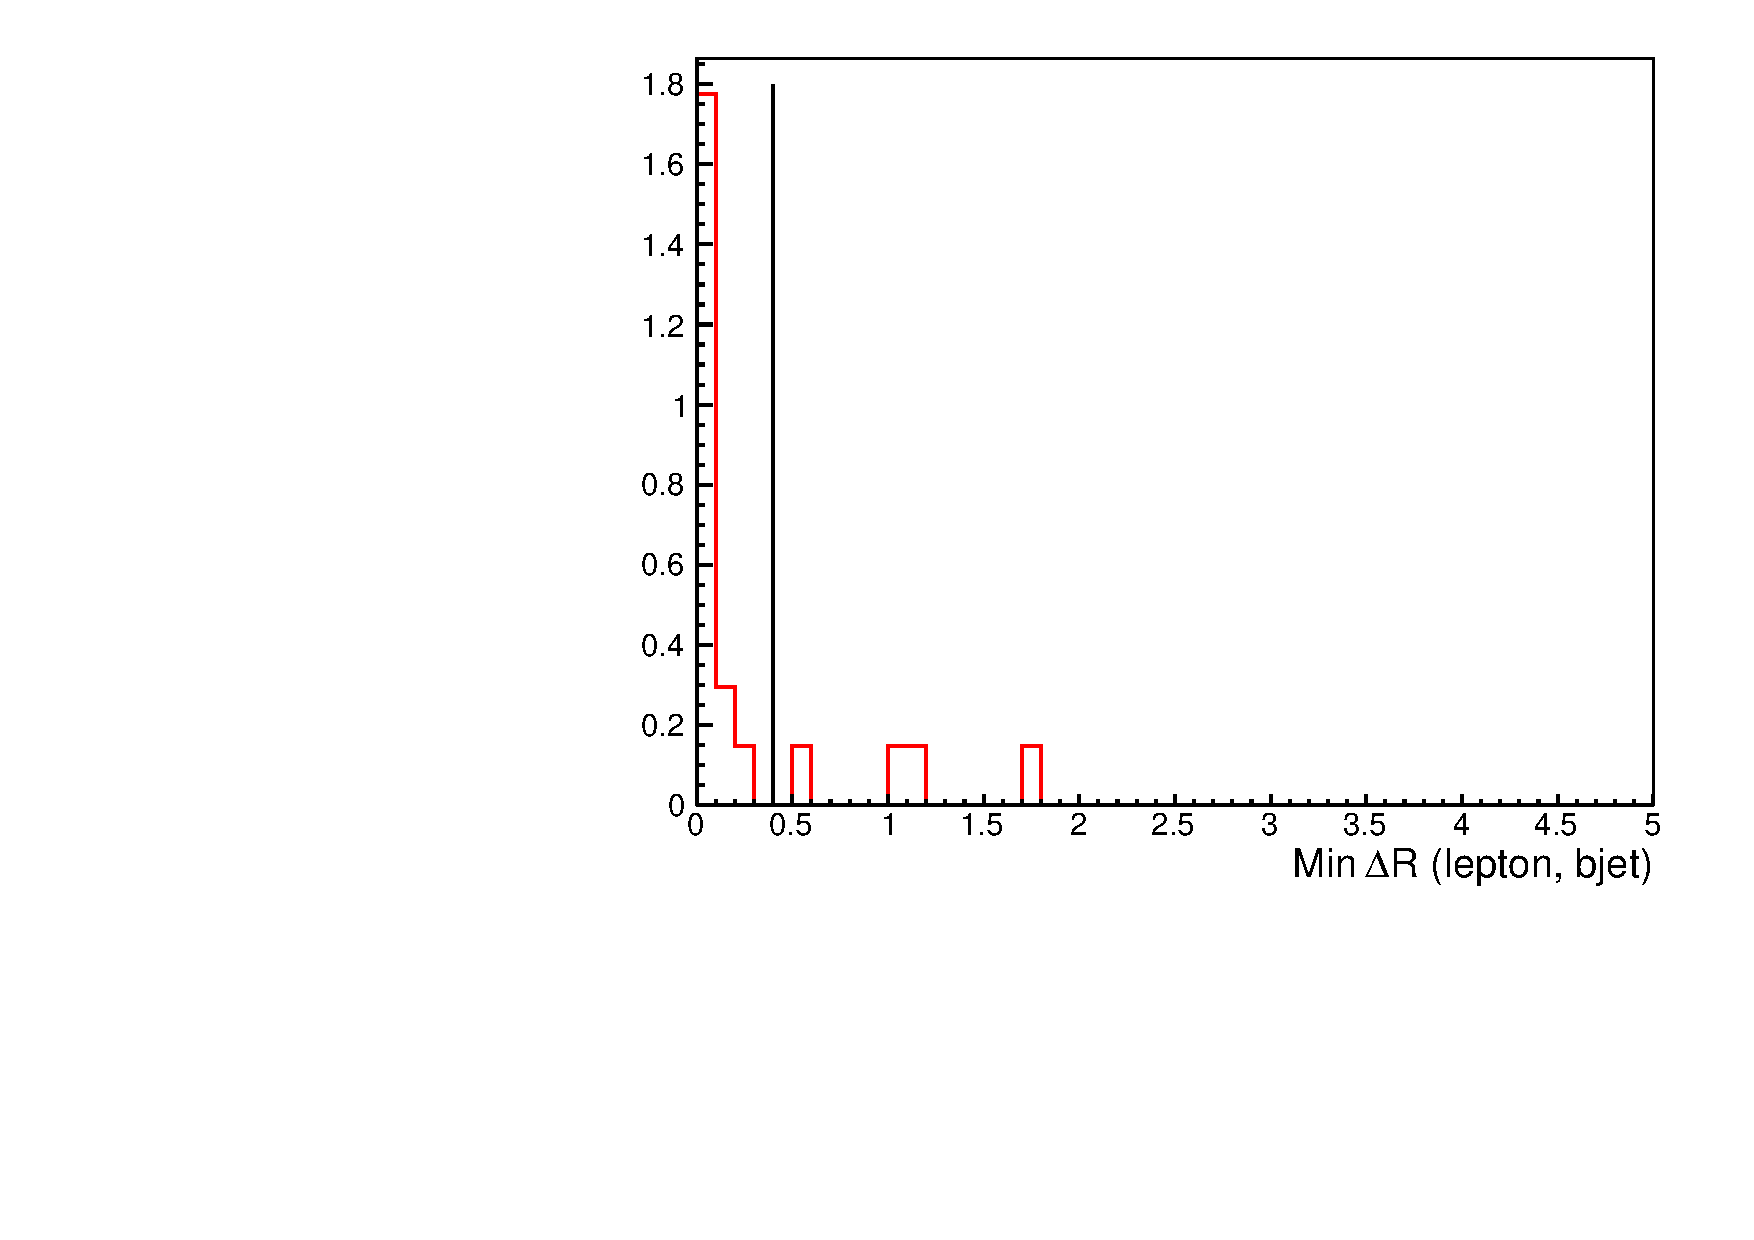
\includegraphics[width=0.6\linewidth, height=0.4\linewidth]{figs/bjetlepton.pdf}
\caption{ Minimum $\Delta R$ between the lepton and the b-tag jet in \ttbar decays.\label{fig:ttbar_residual}}
\end{center}
\end{figure}




 




